\section{Preliminary} \label{sec:prelim}

\subsection{STT-RAM Cell Basics}
STT-RAM uses MTJ as the memory storage and leverages the difference in magnetic directions to represent the memory bit.  As shown in Fig.~\ref{fig:sttcell}, MTJ usually contains two ferromagnetic layers.  One ferromagnetic layer is has fixed magnetization direction and it is called the reference layer, while the other layer has a free magnetization direction that can be changed by passing a write current and it is called the free layer. The relative magnetization direction of two ferromagnetic layers determines the resistance of MTJ.  If two ferromagnetic layers have the parallel directions, the resistance of MTJ is low, indicating a ``1" state; if two layers have anti-parallel directions, the resistance of MTJ is high, indicating a ``0" state.

As shown in Figure~\ref{fig:sttcell}, there are two possible schemes to stack MTJ atop access NMOS transistor. Conventionally, the free layer of MTJ is connected to bitline~(BJ). In that scheme, when writing ``1" state into STT-RAM cells, positive voltage difference is established between BL and SL and the switching current required is $I_{c}(AP\rightarrow P)$; when writing ``0" state, negative voltage difference is established between BL and SL and the switching current required is $I_{c}(P\rightarrow AP)$. While the reverse connection scheme was proposed in~\cite{STTRAM:Qualcomm09} where the free layer of MTJ is connected to the drain of NMOS instead of BL. \cite{STTRAM:Qualcomm09} argues that $I_{c}(P\rightarrow AP)$ is normally significantly larger than $I_{c}(AP\rightarrow P)$~\cite{STTRAM:APL05,STTRAM:PRB05} due to the inherent torque asymmetry of MTJ. But the SL-to-BL current is much smaller than the BL-to-SL current under the same wordline voltage and voltage difference between BL and SL because the body effect of access transistor degrades the SL-to-BL current remarkably. Thus reserving connection scheme can relax the sizing requirement on access transistor, which results in more compact STT-RAM cell size. However, device-level efforts have been put to improve the asymmetry of switching characteristic of MTJ and $I_{c}(AP\rightarrow P)$ slightly larger than $I_{c}(P\rightarrow AP)$ was even demonstrated in~\cite{STTRAM:Grandis07}. In our work, we always choose the MJT connection scheme that is responsible for relaxed sizing requirement on access transistor.

\begin{figure}[t]
  \centering
  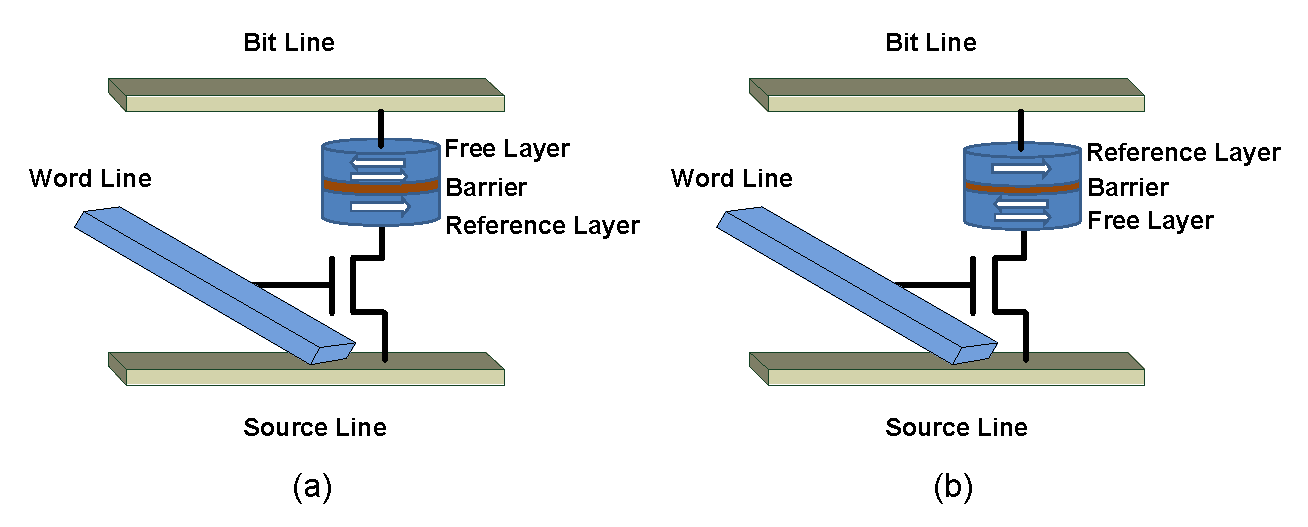
\includegraphics[width=3.5in]{fig/sttramcell.eps}
  \caption{Demonstration of a STT-RAM cell: (a) Conventional connection scheme; (b) Reverse connection scheme.}
  \label{fig:sttcell}
\end{figure}

Another important metric for an MTJ is the tunnel magnetoresistance~(TMR) which is defined as,
\begin{equation}
TMR = \frac{R_{AP}-R_{P}}{R_{P}}
\label{eqn:tmr}
\end{equation}
where ${R_{AP}}$ is the electrical resistance in the anti-parallel state, whereas ${R_{P}}$ is the resistance in the parallel state. A large TMR means big gap between low resistance state~(LRS) and high resistance state~(HRS), which could essentially brings faster read sensing latency or relaxes the constraint for sense amplifier design. It's critical to introduce an equivalent metric for a STT-RAM cell which contains both the MTJ and the access transistor. Similarly the cell TMR~(CTMR) is defined as,
\begin{equation}
CTMR = \frac{R_{cell,AP}-R_{cell,P}}{R_{cell,P}}
\label{eqn:ctmr}
\end{equation}
where $R_{cell,AP}$ is the total cell resistance when the MTJ is in the anti-parallel state, whereas $R_{cell,P}$ is the total cell resistance when the MTJ is in the parallel state. CTMR can be expressed by another equation,
\begin{equation}
CTMR = \frac{I_{P}-I_{AP}}{I_{AP}}
\label{eqn:ctmr2}
\end{equation}
where ${I_{AP}}$ and ${I_{P}}$ are the currents for reading ``0" state and ``1" state. If we ignore the resistance difference of the access transistor for reading ``0" state and ``1" state. CTMR can be interpreted as,
\begin{equation}
CTMR = \frac{R_{AP}-R_{P}}{R_{P}+R_{NMOS}} = \frac{R_{AP}-R_{P}}{R_{P}+\frac{C}{W}}
\label{eqn:ctmr3}
\end{equation}
where $R_{NMOS}$ is the equvalent resistance of access NMOS transistor and $W$ is the transistor width, $C$ is a constant related to the wordline voltage and threshold voltage of the transistor. From equation~\ref{eqn:ctmr3} we can conclude that sizing up the access transistor will make CTMR close to the inherent TMR of MTJ.

\subsection{Write current versus write pulse width trade-off}
The current amplitude required to reverse the direction of the free ferromagnetic layer is determined by a lot of factors such as material property, device geometry and importantly the write pulse duration. Generally, the longer the write pulse is applied, the less the switching current is needed to switch the MTJ state. Three distinct switching modes were identified~\cite{STTRAM:JAP07} according to the operating range of switching pulse width $\tau$: thermal activation ($\tau>20ns$), processional switching ($\tau<3ns$) and dynamic reversal ($3ns<\tau<20ns$). 

\begin{figure}[t]
  \centering
  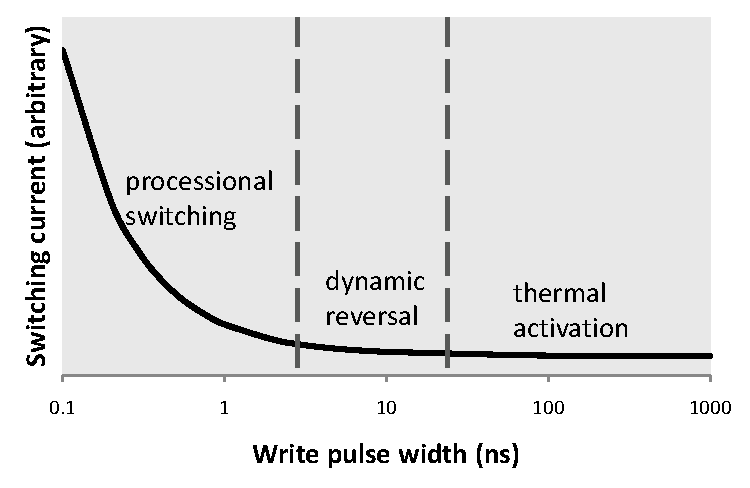
\includegraphics[width=3in]{fig/IcWt.eps}
  \caption{Demonstration of three switching phases: thermal activation, dynamic reversal and precessional switching.}
  \label{fig:IcWt}
\end{figure}

The relationship between switching current current $J_{c}$ and write pulse width $\tau$ was characterized by an analytical model in~\cite{STTRAM:IEDM09}. The equations are listed as follows,
\begin{eqnarray}
J_{c,TA}(\tau) &=& J_{c0}\{1- (\frac{k_{B}T}{E_{b}})ln(\frac{\tau}{\tau_{0}})\} \label{eqn:jcta} \\
J_{c,PS}(\tau) &=& J_{c0}+ \frac{C}{\tau^{\gamma}} \label{eqn:jcps} \\
J_{c,DR}(\tau) &=& \frac{J_{c,TA}(\tau)+J_{c,PS}(\tau)e^{-k(\tau - \tau_{c})}}{1+e^{-k(\tau - \tau_{c})}} \label{eqn:jcdr} 
\end{eqnarray}  
where $J_{c,TA}$, $J_{c,PS}$, $J_{c,DR}$ are the switching current density for thermal activation, precessional switching and dynamic reversal. $J_{c0}$ is the critical switching current density. $k_{B}$ is the Boltzmann constant, $T$ is the temperature, $E_{b}$ is the thermal barrier, and $\tau_{0}$ is inverse of the attempt frequency. $C$, $\gamma$, $k$, and $\tau_{c}$ are fitting constants. Based on the observation from Figure~\ref{fig:IcWt} and analysis of the analytical model,  we found very different switching characteristics in the three switching modes. For example, in thermal activation mode, the required switching current decrease very slowly even we increase the write pulse width by orders of magnitude, thus short write pulse width is more favorable in this regime because reducing write pulse can reduce both write latency and energy without much penalty on read latency and energy. While in processional switching, write current goes up rapidly if we further reduce write pulse width, therefore minimum write energy of the MTJ is achieved at some particular write pulse width in this regime. Consequently, this paper will focus on the exploration of write pulse width in processional switching and dynamic reversal to optimize for different design goals.

\subsection{Perpendicular MTJ}
